\documentclass[twoside]{article}
\usepackage[utf8]{inputenc}
%\usepackage[uebung, answers]{tumbgdm}
\usepackage[klausur]{tumbgdm}
\usepackage{lecturesetup}
\usepackage{pdfpages}
%\nummerUebungsblatt{6}
%\nummerErsteFrage{14}
\klausurTitle{Sample Exam Computational Foundations II \\(LRG0061, Summer Term 2022)}
%\LearningOutcome{
%We are warming up with C/C++ programming environments.
%}
\lstset{numbers=left, stepnumber=1}
\begin{document}

\maketitle
% 90 points for 90 minutes
\evaluationtable

\clearpage

\begin{task}{Multiple Choice}{5}{}
  Answer the following questions with yes or no. \\
  \emph{A wrong answer is counted as -1, a correct answer is counted as +1, an answer not given is counted as 0 (if you don't know the answer it is smarter not to give an answer!). If you reach more than 5 points, the points will become bonus points, if you reach less than 0 points, the result is 0 points.}
  \vspace{2cm}
  
\begin{mclist}
%  \mcquestion{In MATLAB, subsets of data can be created with slicing.}{X}{}{}
% \mcquestion{In MATLAB, one needs to allocate memory for an object before creating or using it using malloc and free.}{}{X}{}
% \mcquestion{For arbitrary large $n$, an algorithm of runtime complexity $O(n)$ will become faster than an algorithm of $O(n^2)$.}{X}{}{Of course}
% \mcquestion{The SDL libraries are a collection of linear algebra routines such that we can easily solve numeric problems in C++.}{}{X}{SDL = Simple Direct Media Layer = simple GUI framework.}
% \mcquestion{MATLAB is a compiled language generating native executables.}{}{X}{}
% \mcquestion{C++ is a compiled language generating native executables.}{X}{}{}
  % \mcquestion{A complete binary tree with depth $n$ has $2^n$ leaf nodes.}{X}{}{}
  \mcquestion{IEEE standard for floating point numbers (754) supports certain special values like infinity}{X}{}{}
  \mcquestion{A 3-bit unsigned integer ranges from including 0 to including 7.}{X}{}{}
  \mcquestion{When multiplying two 8-bit numbers, the result can be held in 8 bit.}{}{X}{}
  \mcquestion{For computing the shortest path between all nodes of a graph, one typically runs Dijkstra with each node as the starting point}{}{X}{}
  \mcquestion{In network coding, the transmission capacity can be higher than in network routing.}{X}{}{}
  \mcquestion{A sixth question}{}{}{}
  \mcquestion{A seventh question}{}{}{}  
  \end{mclist}

\end{task}
\clearpage
\begin{task}{Combinatorial Circuits}{5}{}
  The following truth table defines a half-adder:

  \begin{tabular}{cc|cc}
    a & b & s & c \\ \hline
    0 & 0 & 0 & 0 \\
    0 & 1 & 1 & 0 \\
    1 & 0 & 1 & 0 \\
    1 & 1 & 0 & 1 \\
    \end{tabular}

  
  \begin{enumerate}
  \item {Give the Sum-of-Products (SOP) representation of the circuit. \vspace*{3cm}}
  \item{Implement (exactly) the SOP for the output $s$.

    
    \vspace*{6cm}}
  \item{Give the complete truth table of the following circuit, where HA stands for an instance of the half adder.

    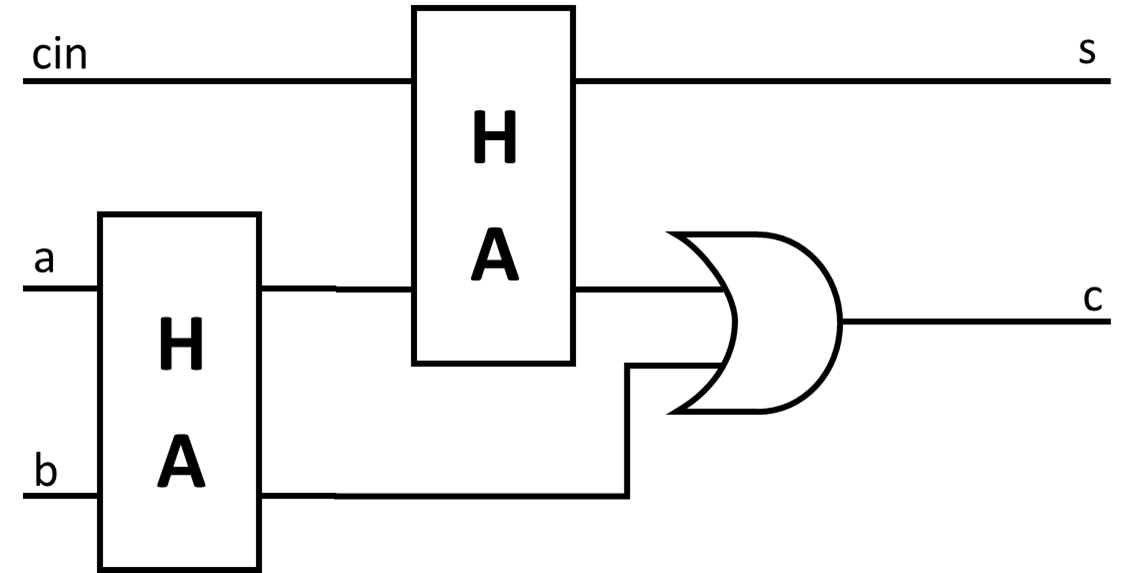
\includegraphics[width=.5\textwidth]{gfx/halfadder.png}
}
    \clearpage
    \item{Using ICs of a Full Adder and a Half Adder, build a 2-bit addition circuit (4 inputs, 5 outputs) and give the truth table for rows where the first bit of the first input is 0.}
  \end{enumerate}
  
\end{task}
\clearpage
\begin{task}{Quadrature Phase Shift Keying}{5}{}
  The idea of the QPSK phase shift keying is that various phases represent different symbols, such that two bit are transmitted at the same time.

  \begin{enumerate}
  \item{Given a bitstring of 11010011, draw the modulation waveform in the following diagram and mark all keypoints (e.g., points where the waveform intersects the organizational lines) for better readability. Each symbol of two bit shall be transmitted with one roundtrip of the wave.

    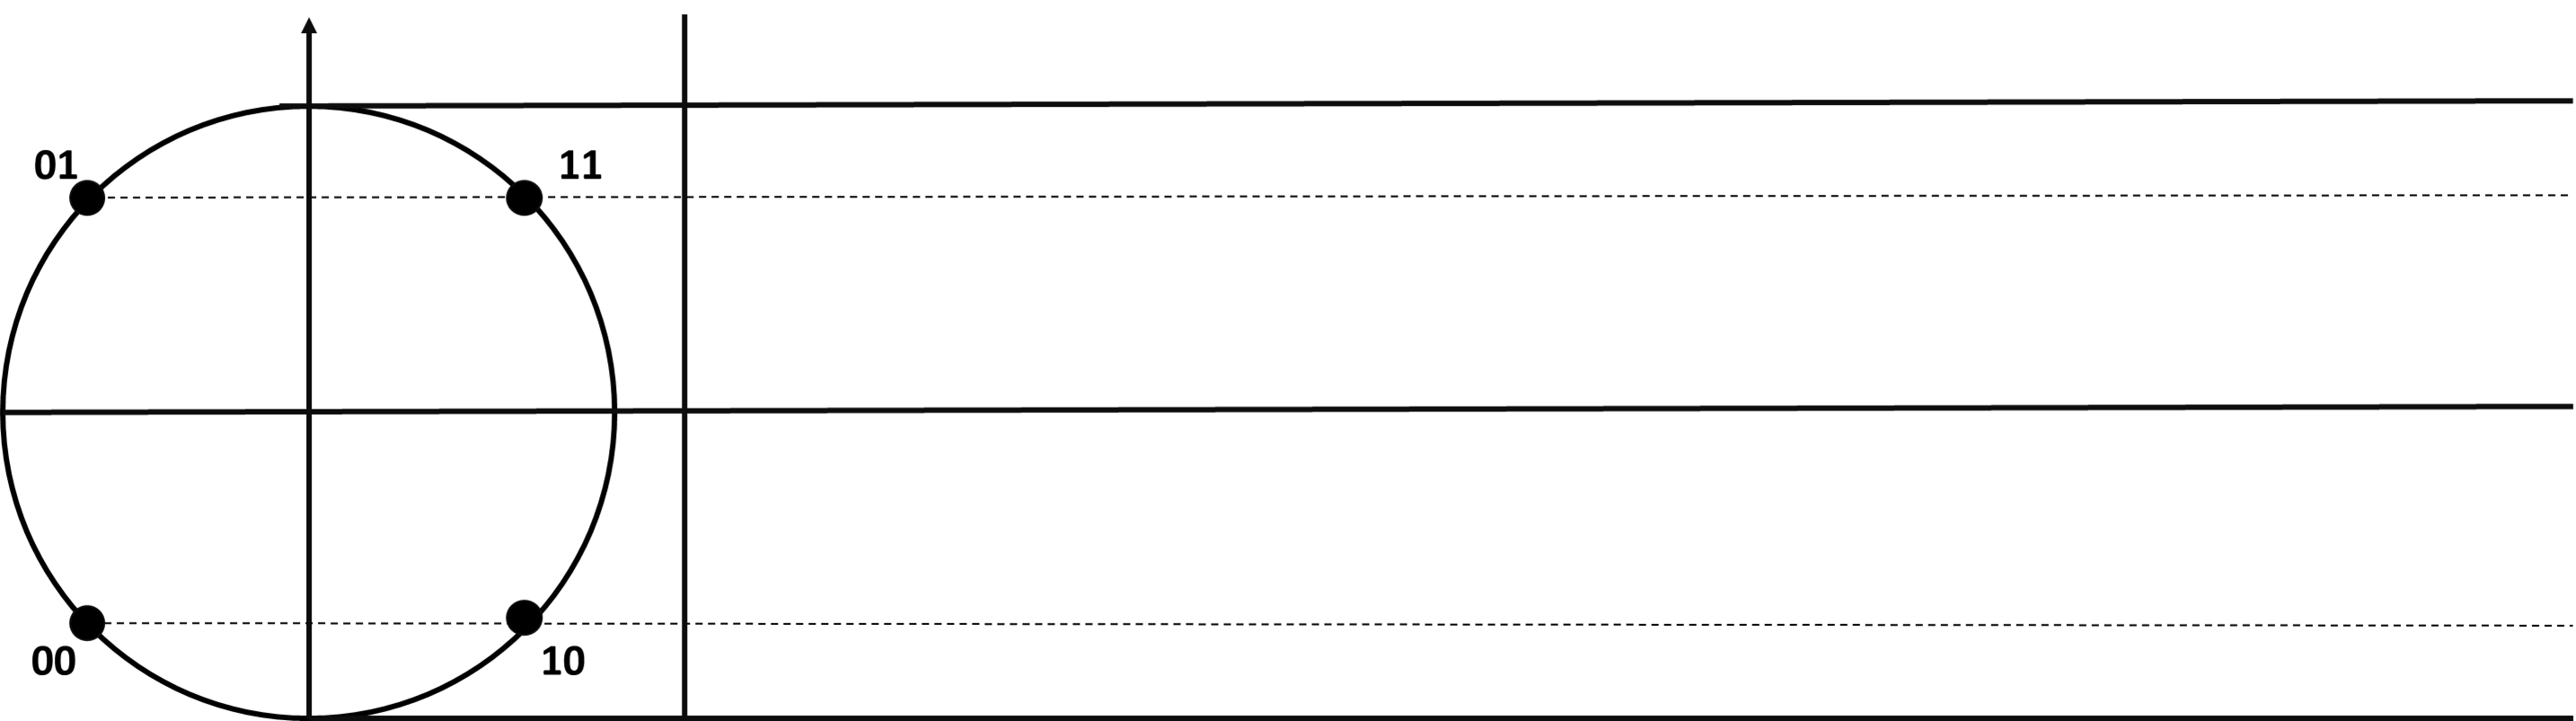
\includegraphics[width=\textwidth]{gfx/qpsk.png}

  }
  \item{
    
  }
    \end{enumerate}
\end{task}

\begin{task}{Socket API}{5}{}
  The Berkeley socket API is still the basic operating system interface for networking. It provides (among others) the following functions: socket, listen, connect, accept, shutdown, close, send and recv.
  
  \begin{enumerate}
  \item{ List the required socket API functions in the right order to connect to a server. \vspace*{2cm}}
  \item{Describe the difference between TCP/IP and UDP/IP in a single sentence.}
    \item{What is the API function shutdown good for?}
    \end{enumerate}
  \end{task}
\clearpage
\begin{task}{Broadcast Routing}{5}{}
  In Broadcast Routing, a message si sent to all neighbors in the network graph such that it ultimately reaches the destination.
  \begin{enumerate}
  \item{What is redundancy (single sentence)?\vspace*{2cm}}
  \item{What is implosion (single sentence)?\vspace*{2cm}}
  \item{How does the hop count infuence redundancy?\vspace*{2cm}}
  \item{Given a hop-count smaller than the network diameter, not all nodes can be reached. Why?\vspace*{2cm}}
    \end{enumerate}
  
  \end{task}
\clearpage
\begin{task}{Shortest Paths}{5}{}
  \begin{enumerate}
  \item {How does Dijkstra store shortest path information? \vspace*{2cm}}
  \item{In which odrder does the Priority Queue give the gray vertices from the Dijkstra algorithm?}
    \end{enumerate}
  
\end{task}
\end{document}
